% Options for packages loaded elsewhere
\PassOptionsToPackage{unicode}{hyperref}
\PassOptionsToPackage{hyphens}{url}
\PassOptionsToPackage{dvipsnames,svgnames,x11names}{xcolor}
%
\documentclass[
  letterpaper,
  DIV=11,
  numbers=noendperiod]{scrreport}

\usepackage{amsmath,amssymb}
\usepackage{lmodern}
\usepackage{iftex}
\ifPDFTeX
  \usepackage[T1]{fontenc}
  \usepackage[utf8]{inputenc}
  \usepackage{textcomp} % provide euro and other symbols
\else % if luatex or xetex
  \usepackage{unicode-math}
  \defaultfontfeatures{Scale=MatchLowercase}
  \defaultfontfeatures[\rmfamily]{Ligatures=TeX,Scale=1}
\fi
% Use upquote if available, for straight quotes in verbatim environments
\IfFileExists{upquote.sty}{\usepackage{upquote}}{}
\IfFileExists{microtype.sty}{% use microtype if available
  \usepackage[]{microtype}
  \UseMicrotypeSet[protrusion]{basicmath} % disable protrusion for tt fonts
}{}
\makeatletter
\@ifundefined{KOMAClassName}{% if non-KOMA class
  \IfFileExists{parskip.sty}{%
    \usepackage{parskip}
  }{% else
    \setlength{\parindent}{0pt}
    \setlength{\parskip}{6pt plus 2pt minus 1pt}}
}{% if KOMA class
  \KOMAoptions{parskip=half}}
\makeatother
\usepackage{xcolor}
\setlength{\emergencystretch}{3em} % prevent overfull lines
\setcounter{secnumdepth}{5}
% Make \paragraph and \subparagraph free-standing
\ifx\paragraph\undefined\else
  \let\oldparagraph\paragraph
  \renewcommand{\paragraph}[1]{\oldparagraph{#1}\mbox{}}
\fi
\ifx\subparagraph\undefined\else
  \let\oldsubparagraph\subparagraph
  \renewcommand{\subparagraph}[1]{\oldsubparagraph{#1}\mbox{}}
\fi


\providecommand{\tightlist}{%
  \setlength{\itemsep}{0pt}\setlength{\parskip}{0pt}}\usepackage{longtable,booktabs,array}
\usepackage{calc} % for calculating minipage widths
% Correct order of tables after \paragraph or \subparagraph
\usepackage{etoolbox}
\makeatletter
\patchcmd\longtable{\par}{\if@noskipsec\mbox{}\fi\par}{}{}
\makeatother
% Allow footnotes in longtable head/foot
\IfFileExists{footnotehyper.sty}{\usepackage{footnotehyper}}{\usepackage{footnote}}
\makesavenoteenv{longtable}
\usepackage{graphicx}
\makeatletter
\def\maxwidth{\ifdim\Gin@nat@width>\linewidth\linewidth\else\Gin@nat@width\fi}
\def\maxheight{\ifdim\Gin@nat@height>\textheight\textheight\else\Gin@nat@height\fi}
\makeatother
% Scale images if necessary, so that they will not overflow the page
% margins by default, and it is still possible to overwrite the defaults
% using explicit options in \includegraphics[width, height, ...]{}
\setkeys{Gin}{width=\maxwidth,height=\maxheight,keepaspectratio}
% Set default figure placement to htbp
\makeatletter
\def\fps@figure{htbp}
\makeatother

\KOMAoption{captions}{tableheading}
\makeatletter
\@ifpackageloaded{tcolorbox}{}{\usepackage[many]{tcolorbox}}
\@ifpackageloaded{fontawesome5}{}{\usepackage{fontawesome5}}
\definecolor{quarto-callout-color}{HTML}{909090}
\definecolor{quarto-callout-note-color}{HTML}{0758E5}
\definecolor{quarto-callout-important-color}{HTML}{CC1914}
\definecolor{quarto-callout-warning-color}{HTML}{EB9113}
\definecolor{quarto-callout-tip-color}{HTML}{00A047}
\definecolor{quarto-callout-caution-color}{HTML}{FC5300}
\definecolor{quarto-callout-color-frame}{HTML}{acacac}
\definecolor{quarto-callout-note-color-frame}{HTML}{4582ec}
\definecolor{quarto-callout-important-color-frame}{HTML}{d9534f}
\definecolor{quarto-callout-warning-color-frame}{HTML}{f0ad4e}
\definecolor{quarto-callout-tip-color-frame}{HTML}{02b875}
\definecolor{quarto-callout-caution-color-frame}{HTML}{fd7e14}
\makeatother
\makeatletter
\makeatother
\makeatletter
\@ifpackageloaded{bookmark}{}{\usepackage{bookmark}}
\makeatother
\makeatletter
\@ifpackageloaded{caption}{}{\usepackage{caption}}
\AtBeginDocument{%
\ifdefined\contentsname
  \renewcommand*\contentsname{Table of contents}
\else
  \newcommand\contentsname{Table of contents}
\fi
\ifdefined\listfigurename
  \renewcommand*\listfigurename{List of Figures}
\else
  \newcommand\listfigurename{List of Figures}
\fi
\ifdefined\listtablename
  \renewcommand*\listtablename{List of Tables}
\else
  \newcommand\listtablename{List of Tables}
\fi
\ifdefined\figurename
  \renewcommand*\figurename{Figure}
\else
  \newcommand\figurename{Figure}
\fi
\ifdefined\tablename
  \renewcommand*\tablename{Table}
\else
  \newcommand\tablename{Table}
\fi
}
\@ifpackageloaded{float}{}{\usepackage{float}}
\floatstyle{ruled}
\@ifundefined{c@chapter}{\newfloat{codelisting}{h}{lop}}{\newfloat{codelisting}{h}{lop}[chapter]}
\floatname{codelisting}{Listing}
\newcommand*\listoflistings{\listof{codelisting}{List of Listings}}
\makeatother
\makeatletter
\@ifpackageloaded{caption}{}{\usepackage{caption}}
\@ifpackageloaded{subcaption}{}{\usepackage{subcaption}}
\makeatother
\makeatletter
\@ifpackageloaded{tcolorbox}{}{\usepackage[many]{tcolorbox}}
\makeatother
\makeatletter
\@ifundefined{shadecolor}{\definecolor{shadecolor}{rgb}{.97, .97, .97}}
\makeatother
\makeatletter
\makeatother
\ifLuaTeX
  \usepackage{selnolig}  % disable illegal ligatures
\fi
\IfFileExists{bookmark.sty}{\usepackage{bookmark}}{\usepackage{hyperref}}
\IfFileExists{xurl.sty}{\usepackage{xurl}}{} % add URL line breaks if available
\urlstyle{same} % disable monospaced font for URLs
\hypersetup{
  pdftitle={Анализ ресторана},
  pdfauthor={Костыря Владимир},
  colorlinks=true,
  linkcolor={blue},
  filecolor={Maroon},
  citecolor={Blue},
  urlcolor={Blue},
  pdfcreator={LaTeX via pandoc}}

\title{Анализ ресторана}
\author{Костыря Владимир}
\date{14.10.2022}

\begin{document}
\maketitle
\ifdefined\Shaded\renewenvironment{Shaded}{\begin{tcolorbox}[sharp corners, breakable, interior hidden, enhanced, boxrule=0pt, borderline west={3pt}{0pt}{shadecolor}, frame hidden]}{\end{tcolorbox}}\fi

\renewcommand*\contentsname{Table of contents}
{
\hypersetup{linkcolor=}
\setcounter{tocdepth}{2}
\tableofcontents
}
\bookmarksetup{startatroot}

\hypertarget{ux43dux430ux447ux430ux43bux43e-ux440ux430ux431ux43eux442ux44b}{%
\chapter*{Начало
работы}\label{ux43dux430ux447ux430ux43bux43e-ux440ux430ux431ux43eux442ux44b}}
\addcontentsline{toc}{chapter}{Начало работы}

В данном документе проведен анализ подразделения ресторана \#proСчастье

Для анализа были использован отчета из ПО \texttt{iiko} - ``Отчет о
продажах за период''

Стоит отметить, что данные отчеты были предвариельно обработаны и
преведены к единому формату.

\bookmarksetup{startatroot}

\hypertarget{ux43eux442ux447ux435ux442-ux43e-ux43fux440ux43eux434ux430ux436ux430ux445-ux437ux430-ux43fux435ux440ux438ux43eux434}{%
\chapter{Отчет о продажах за
период}\label{ux43eux442ux447ux435ux442-ux43e-ux43fux440ux43eux434ux430ux436ux430ux445-ux437ux430-ux43fux435ux440ux438ux43eux434}}

\hypertarget{ux43cux435ux43dux44e-ux432ux441ux435-ux441ux435ux439ux447ux430ux441-ux445ux43eux440ux43eux448ux43e}{%
\section{Меню ``Все сейчас
хорошо''}\label{ux43cux435ux43dux44e-ux432ux441ux435-ux441ux435ux439ux447ux430ux441-ux445ux43eux440ux43eux448ux43e}}

Начнем с анализа меню ресторана ``Все сейчас хорошо'', так как на данный
момент это является акутальным для нас.

На первом шаге мы загрущзим данные и оставим только те позиции, которые
относятся к меню ``ВСХ''. Все позиции меню данного ресторана обозначены
``ВСХ \textless наименования позиции меню\textgreater{}''.

Посмотрим на структуру данных

\begin{verbatim}
# A tibble: 20 x 20
   date       code  group       food_name count revenue_no_sale sum_sale revenue
   <date>     <chr> <chr>       <chr>     <dbl>           <dbl>    <dbl>   <dbl>
 1 2021-01-05 03905 Кофе для п~ ВСХ  Аме~     2               0        0       0
 2 2021-01-06 03905 Кофе для п~ ВСХ  Аме~     2               0        0       0
 3 2021-01-07 03915 ВСХ  ГАРНИ~ ВСХ  Наг~    10            3000     3000       0
 4 2021-01-07 03828 ВСХ  ЛАПША~ ВСХ  Гре~     6            1860        0    1860
 5 2021-01-07 03875 ВСХ  ПИЦЦА~ ВСХ  Пиц~     2            1200        0    1200
 6 2021-01-07 03842 ВСХ  ПИЦЦА~ ВСХ  Пиц~     2            1200     1200       0
 7 2021-01-07 03838 ВСХ  ПИЦЦА~ ВСХ  Пиц~     1             550      550       0
 8 2021-01-07 03902 ВСХ  САЛАТЫ ВСХ  Цез~     4            1360        0    1360
 9 2021-01-07 03836 ВСХ  СЭНДВ~ ВСХ  Вег~     1             260        0     260
10 2021-01-07 03905 Кофе для п~ ВСХ  Аме~     2               0        0       0
11 2021-01-09 03915 ВСХ  ГАРНИ~ ВСХ  Наг~     7            2100     2100       0
12 2021-01-09 03925 ВСХ  КОФЕ   ВСХ  Аме~     2             240        0     240
13 2021-01-09 03926 ВСХ  КОФЕ   ВСХ  Кап~     2             400        0     400
14 2021-01-09 03927 ВСХ  КОФЕ   ВСХ  Лат~     1             220        0     220
15 2021-01-09 03841 ВСХ  ПИЦЦА~ ВСХ  Пиц~     1             600      600       0
16 2021-01-09 03838 ВСХ  ПИЦЦА~ ВСХ  Пиц~     2            1100     1100       0
17 2021-01-09 03909 Кофе для п~ ВСХ  Кап~     1               0        0       0
18 2021-01-09 03905 Кофе для п~ ВСХ  Аме~     2               0        0       0
19 2021-01-10 03905 Кофе для п~ ВСХ  Аме~     6               0        0       0
20 2021-01-13 03960 ВСХ  ЗАВТР~ ВСХ  Омл~     1             300        0     300
# ... with 12 more variables: cost_one <dbl>, cost_rub <dbl>, food_cost <dbl>,
#   allowance <dbl>, concept <chr>, year <dbl>, month <dbl>, day_number <dbl>,
#   wday <dbl>, discount_rate <dbl>, revenue_end <dbl>, food_cost_end <dbl>
\end{verbatim}

Данные представлены с 2021-01-05 по 2022-09-30. В них содержится 20
колонок. Не все они требуют пояснения.

\begin{tcolorbox}[enhanced jigsaw, colframe=quarto-callout-note-color-frame, leftrule=.75mm, colback=white, arc=.35mm, toprule=.15mm, opacityback=0, bottomrule=.15mm, breakable, left=2mm, rightrule=.15mm]
\begin{minipage}[t]{5.5mm}
\textcolor{quarto-callout-note-color}{\faInfo}
\end{minipage}%
\begin{minipage}[t]{\textwidth - 5.5mm}
Мы детально рассмотрим только те колонки, которые требуют
внимания\end{minipage}%
\end{tcolorbox}

\begin{itemize}
\item
  \textbf{\texttt{code}} - код наменклатуры (SKU) в iiko
\item
  \textbf{\texttt{group}} - группа первого уровня в iiko
\item
  \textbf{\texttt{food\_name}} - наименоание позиции в меню
\item
  \textbf{\texttt{count}} - количество реализованнх SKU в конкретный
  день
\item
  \textbf{\texttt{revenue\_no\_sale}} - выручка без скидок в конкретный
  день по конкретному SKU
\item
  \textbf{\texttt{sum\_sale}} - сумма скидок в рублях
\item
  \textbf{\texttt{revenue}} - выручка за вычитом скидок
\item
  \textbf{\texttt{food\_cost}} - фудкост рассчитанный в iiko
\item
  \textbf{\texttt{allowance}} - наценка
\item
  \textbf{\texttt{discount\_rate}} - размер скидки. Данная переменая
  нужна, чтобы рассчитать реальный фудкост, где не будут учтены наценки
  за обслуживания
\item
  \textbf{\texttt{revenue\_end}} - очищенная выручка от наценок
\item
  \textbf{\texttt{food\_cost\_end}} - расчитанный фудкост
\end{itemize}

Посморим какие группы меню содержатся в наших данных

\begin{verbatim}
# A tibble: 43 x 2
   group                           n
   <chr>                       <int>
 1 ВСХ  КОКТЕЙЛИ                2046
 2 ВСХ  КОФЕ                    1083
 3 ВСХ  ЛИМОНАДЫ                 840
 4 ВСХ  ПИЦЦА НА ОБЫЧНОМ ТЕСТЕ   745
 5 ВСХ  ЛАПША и ПАСТА            684
 6 ВСХ  САЛАТЫ                   566
 7 ВСХ  СУПЫ                     556
 8 ВСХ  ЧАЙ                      530
 9 ВСХ  СЭНДВИЧ РОЛЛЫ            365
10 ВСХ  ПИВО                     301
# ... with 33 more rows
\end{verbatim}

Добавим в наши данные еще одну колонку, которая будет содержать тип
группы: ``Еда'' или ``Бар'' и посмотрим на соотношение количества и
суммы продаж по двум этим параметрам.

\begin{verbatim}
# A tibble: 2 x 3
  group_2 Количество Сумма_продаж
  <chr>        <dbl>        <dbl>
1 Бар         12314.     3491054.
2 Еда          7544.     3042267.
\end{verbatim}

Мы видим, что с 2021-01-05 по 2022-09-30 еды было продано больше, чем
позиций бара. Но по сумме выручки -- цифры сопоставимые.

\hypertarget{ux434ux438ux43dux430ux43cux438ux43aux430-ux43fux440ux43eux434ux430ux436}{%
\subsection*{Динамика
продаж}\label{ux434ux438ux43dux430ux43cux438ux43aux430-ux43fux440ux43eux434ux430ux436}}
\addcontentsline{toc}{subsection}{Динамика продаж}

Посмотрим на динамику продаж по этим двум группам.

\begin{figure}

{\centering 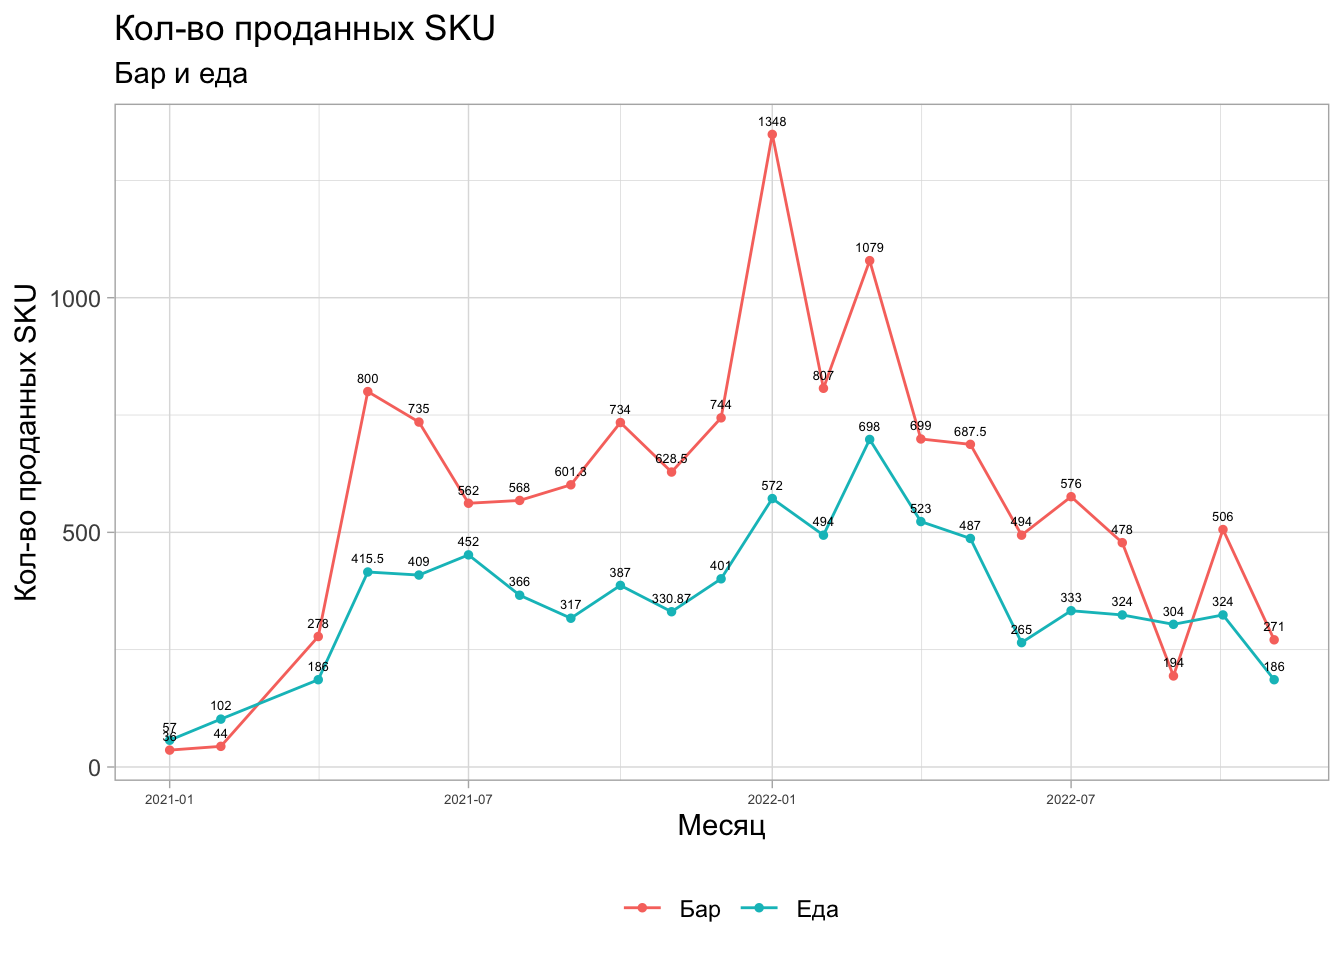
\includegraphics{./intro_files/figure-pdf/unnamed-chunk-6-1.pdf}

}

\end{figure}

\begin{figure}

{\centering 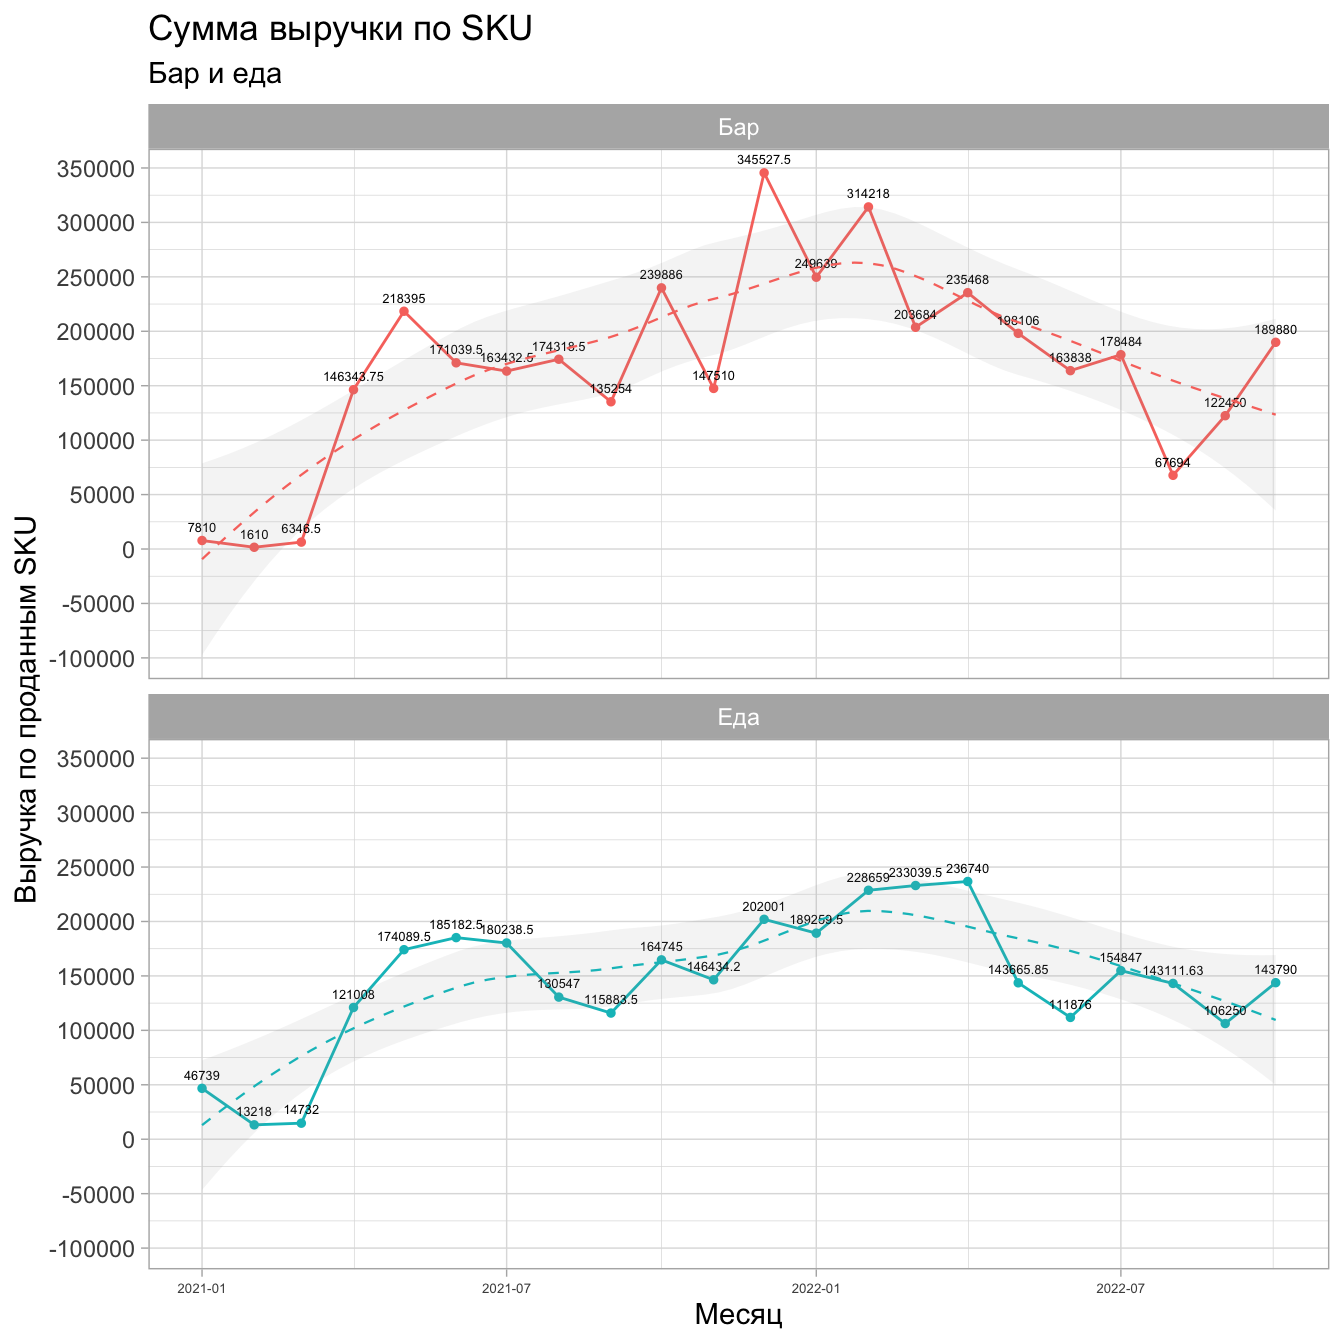
\includegraphics{./intro_files/figure-pdf/unnamed-chunk-7-1.pdf}

}

\end{figure}

Мы видим, что динамика продаж отрицательная. Сложно сделать
окончательные выводы, по имеющимся данным, так как у нас их
недостаточно. Возможно отрицательная динамика -- это всего лишь
сезонность.

При этом стоит отметить, что продажи бара менее вариабельны, чем позиции
по кухне.

\hypertarget{ux434ux438ux43dux430ux43cux438ux43aux430-foodcost-ux43fux43e-ux433ux440ux443ux43fux43fux430ux43c-ux432-ux43cux435ux43dux44e}{%
\subsubsection*{Динамика foodcost по группам в
меню}\label{ux434ux438ux43dux430ux43cux438ux43aux430-foodcost-ux43fux43e-ux433ux440ux443ux43fux43fux430ux43c-ux432-ux43cux435ux43dux44e}}
\addcontentsline{toc}{subsubsection}{Динамика foodcost по группам в
меню}

\begin{figure}

{\centering 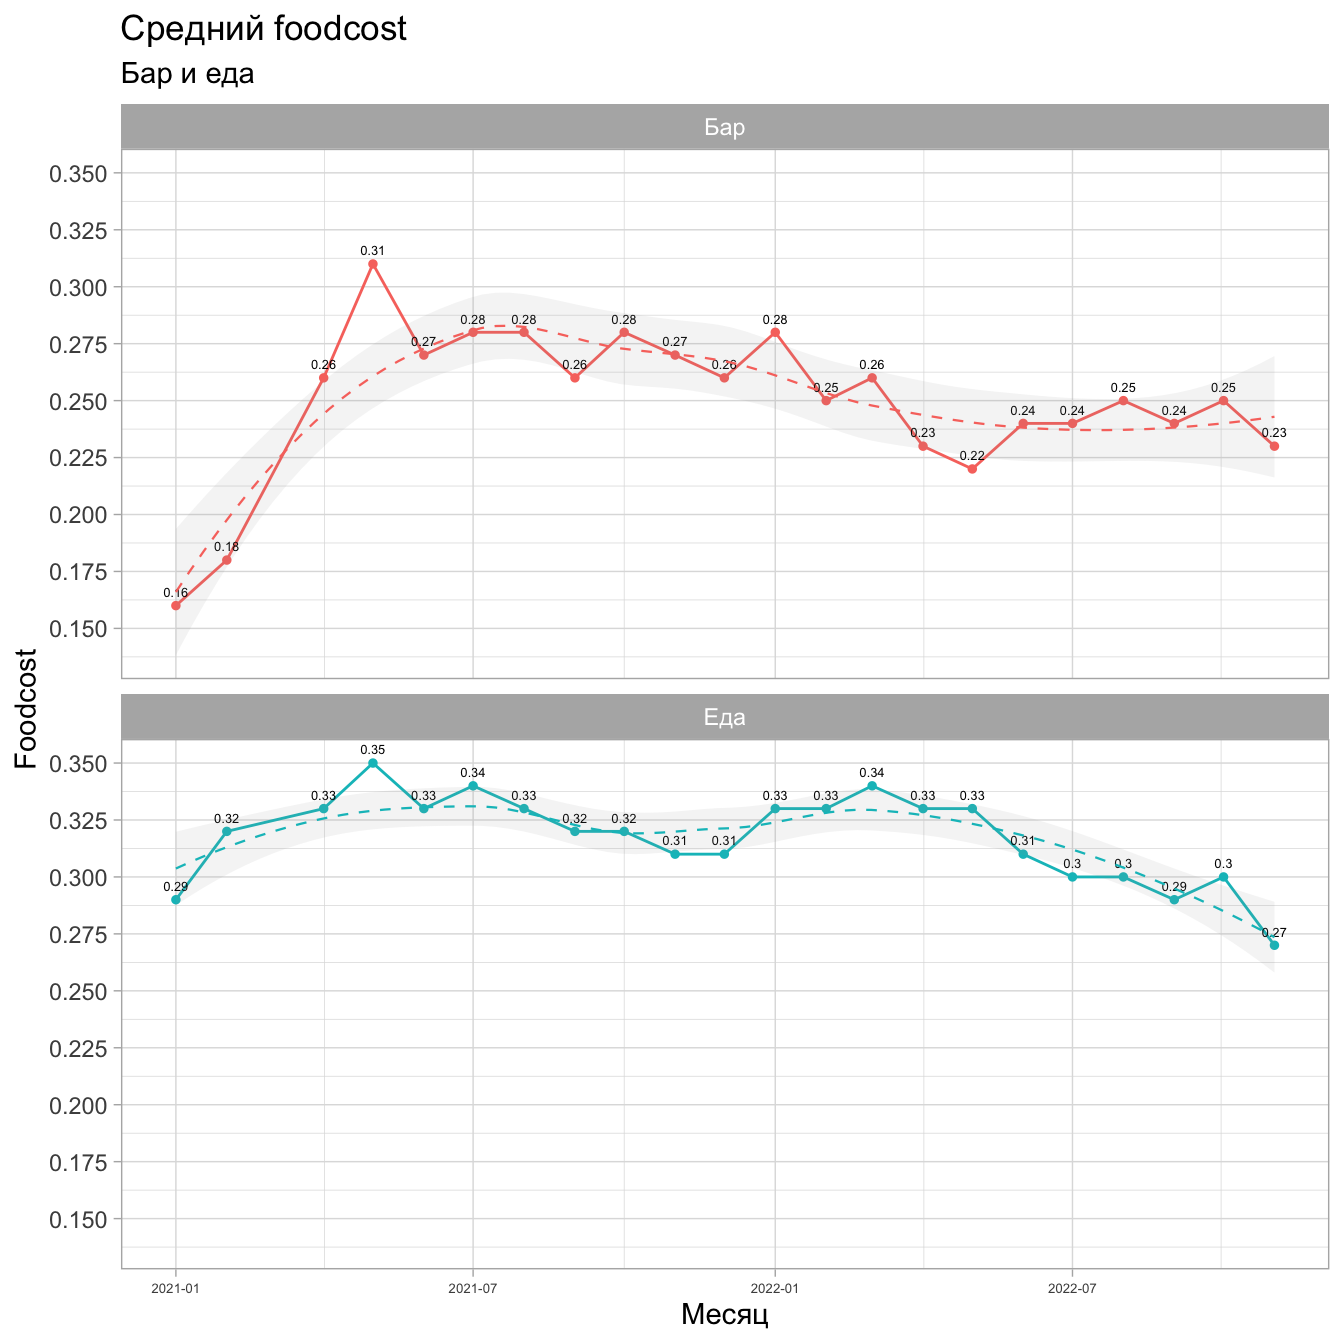
\includegraphics{./intro_files/figure-pdf/unnamed-chunk-8-1.pdf}

}

\end{figure}

\hypertarget{ux43fux43eux43fux443ux43bux44fux440ux43dux44bux435-ux43fux43eux437ux438ux446ux438ux438-ux43cux435ux43dux44e}{%
\subsubsection*{Популярные позиции
меню}\label{ux43fux43eux43fux443ux43bux44fux440ux43dux44bux435-ux43fux43eux437ux438ux446ux438ux438-ux43cux435ux43dux44e}}
\addcontentsline{toc}{subsubsection}{Популярные позиции меню}

Теперь мы можем посмотреть на те позиции, которые наиболее часто
покупают в ``ВСХ''. Нас больше интересует не сама группа, а конкретное
SKU.

Сначала посмотрим на позиции, которые относятся к категории ``Еда''.
Выделим ТОП 50

\begin{figure}

{\centering 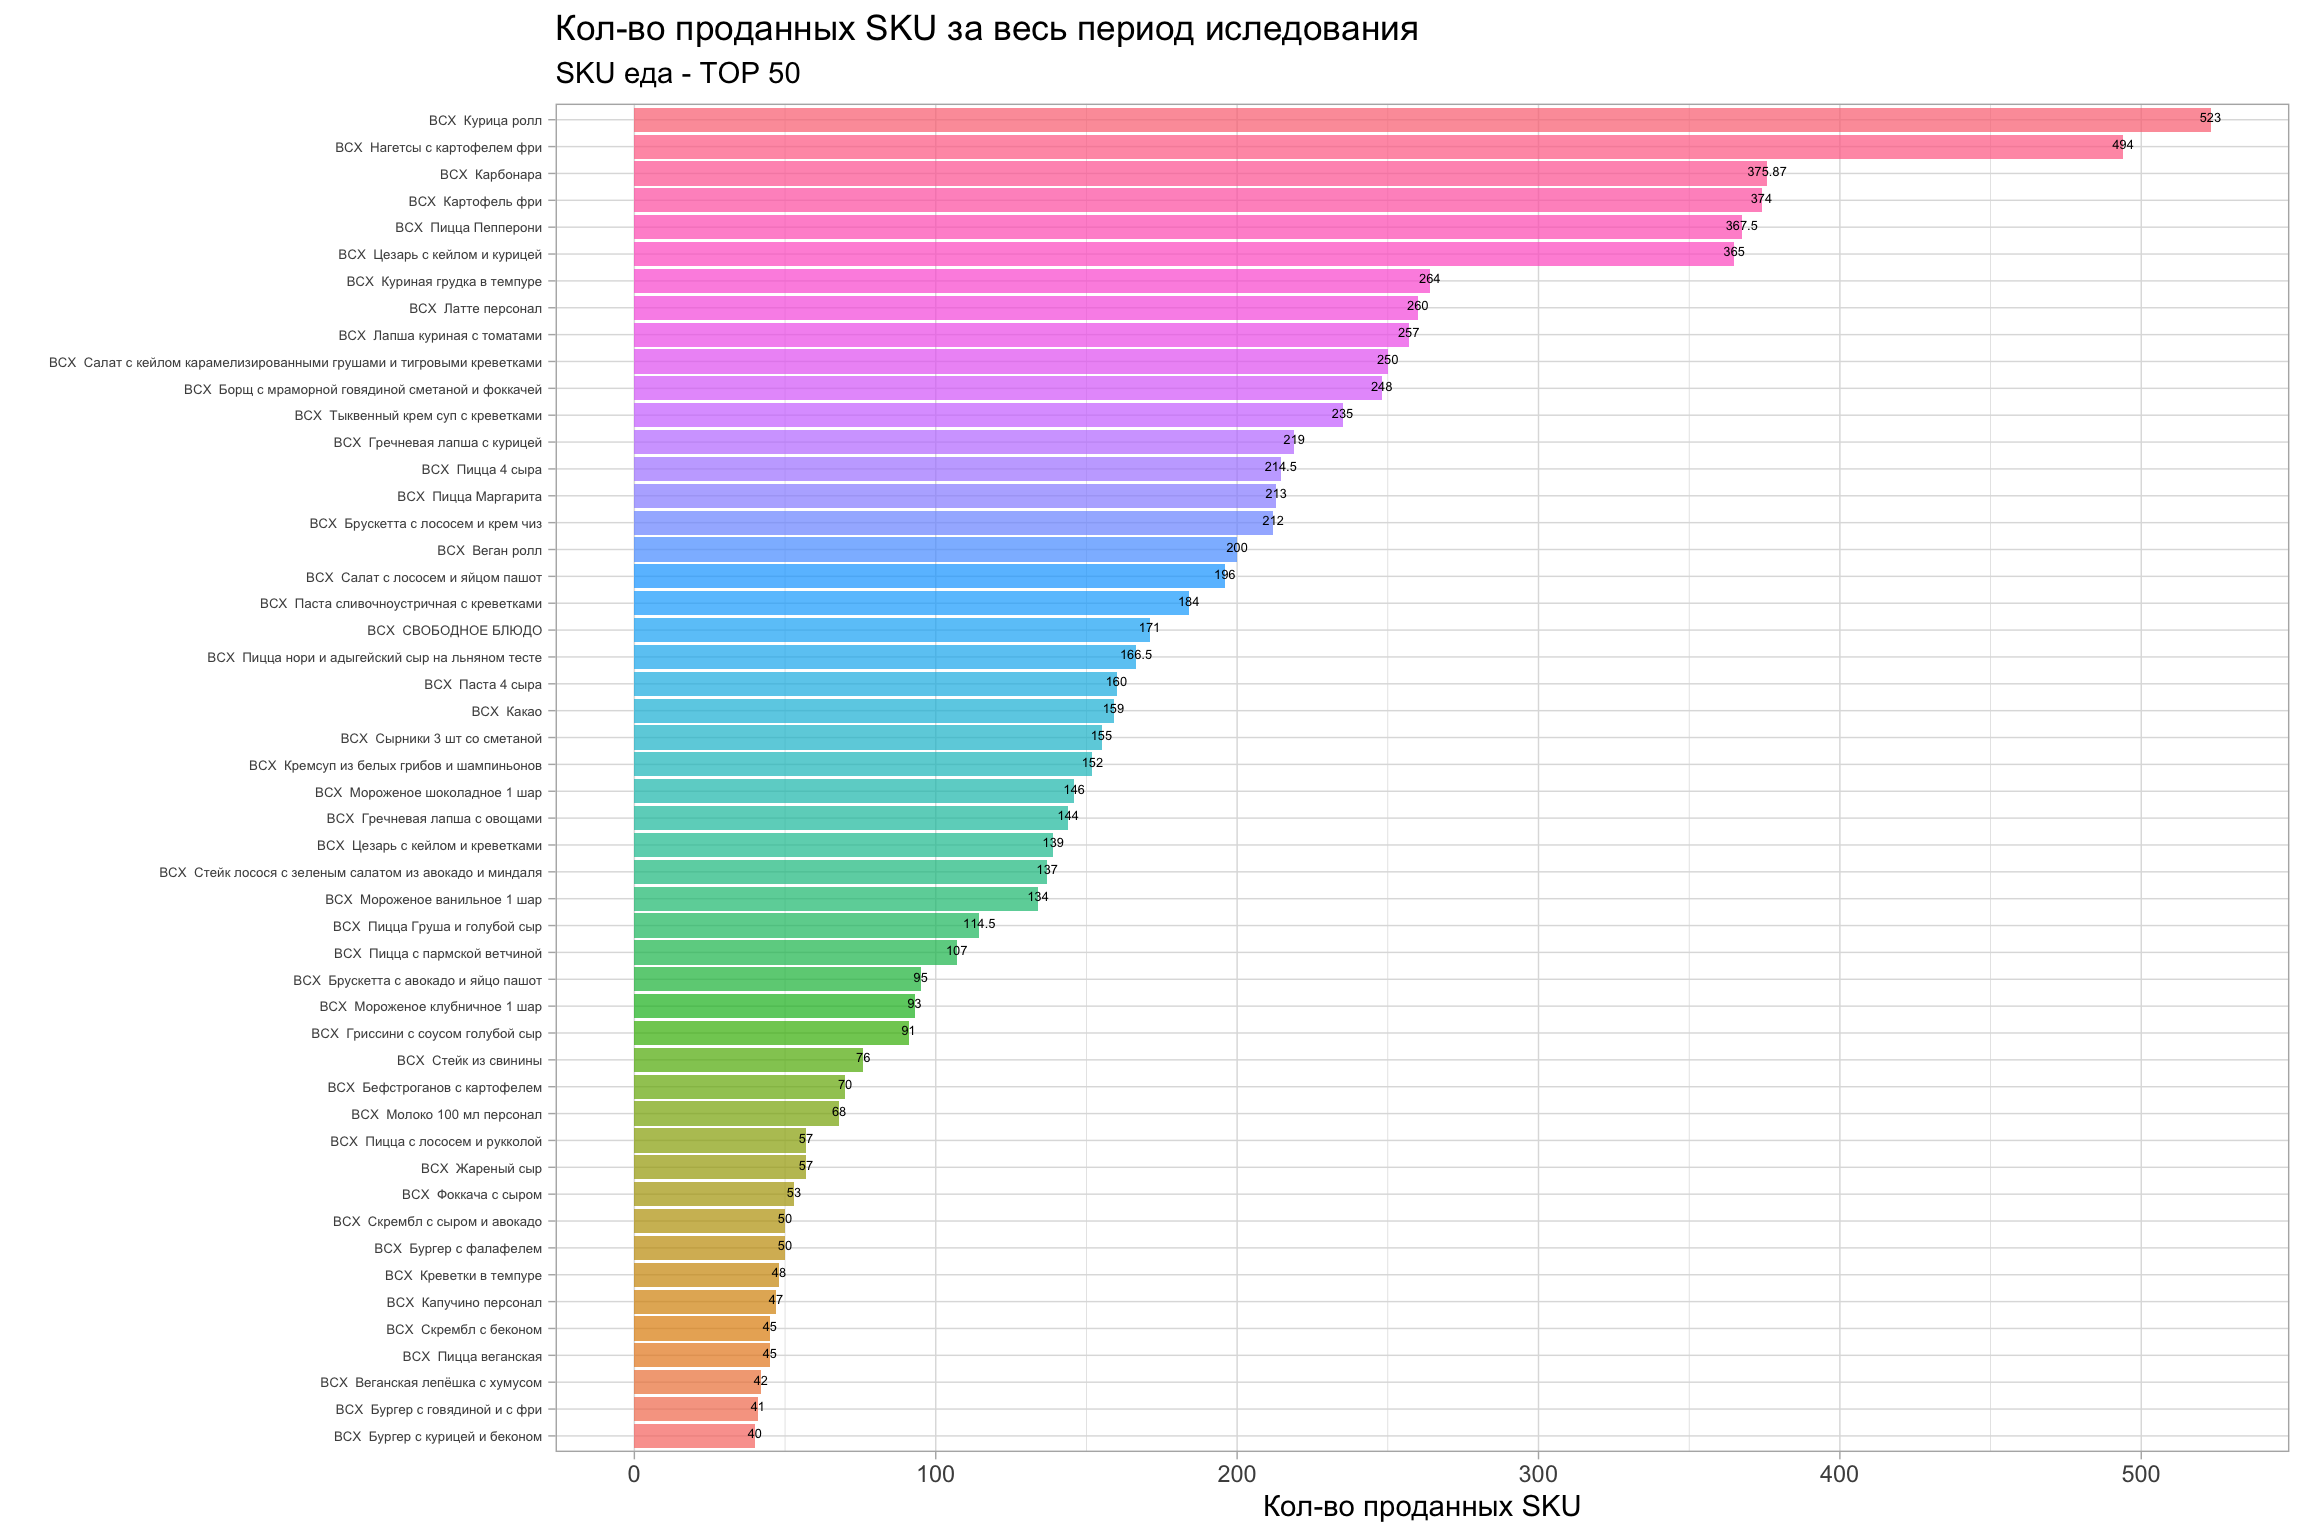
\includegraphics{./intro_files/figure-pdf/unnamed-chunk-9-1.pdf}

}

\end{figure}

Теперь выделим TOP 50 позиций бара:

\begin{figure}

{\centering 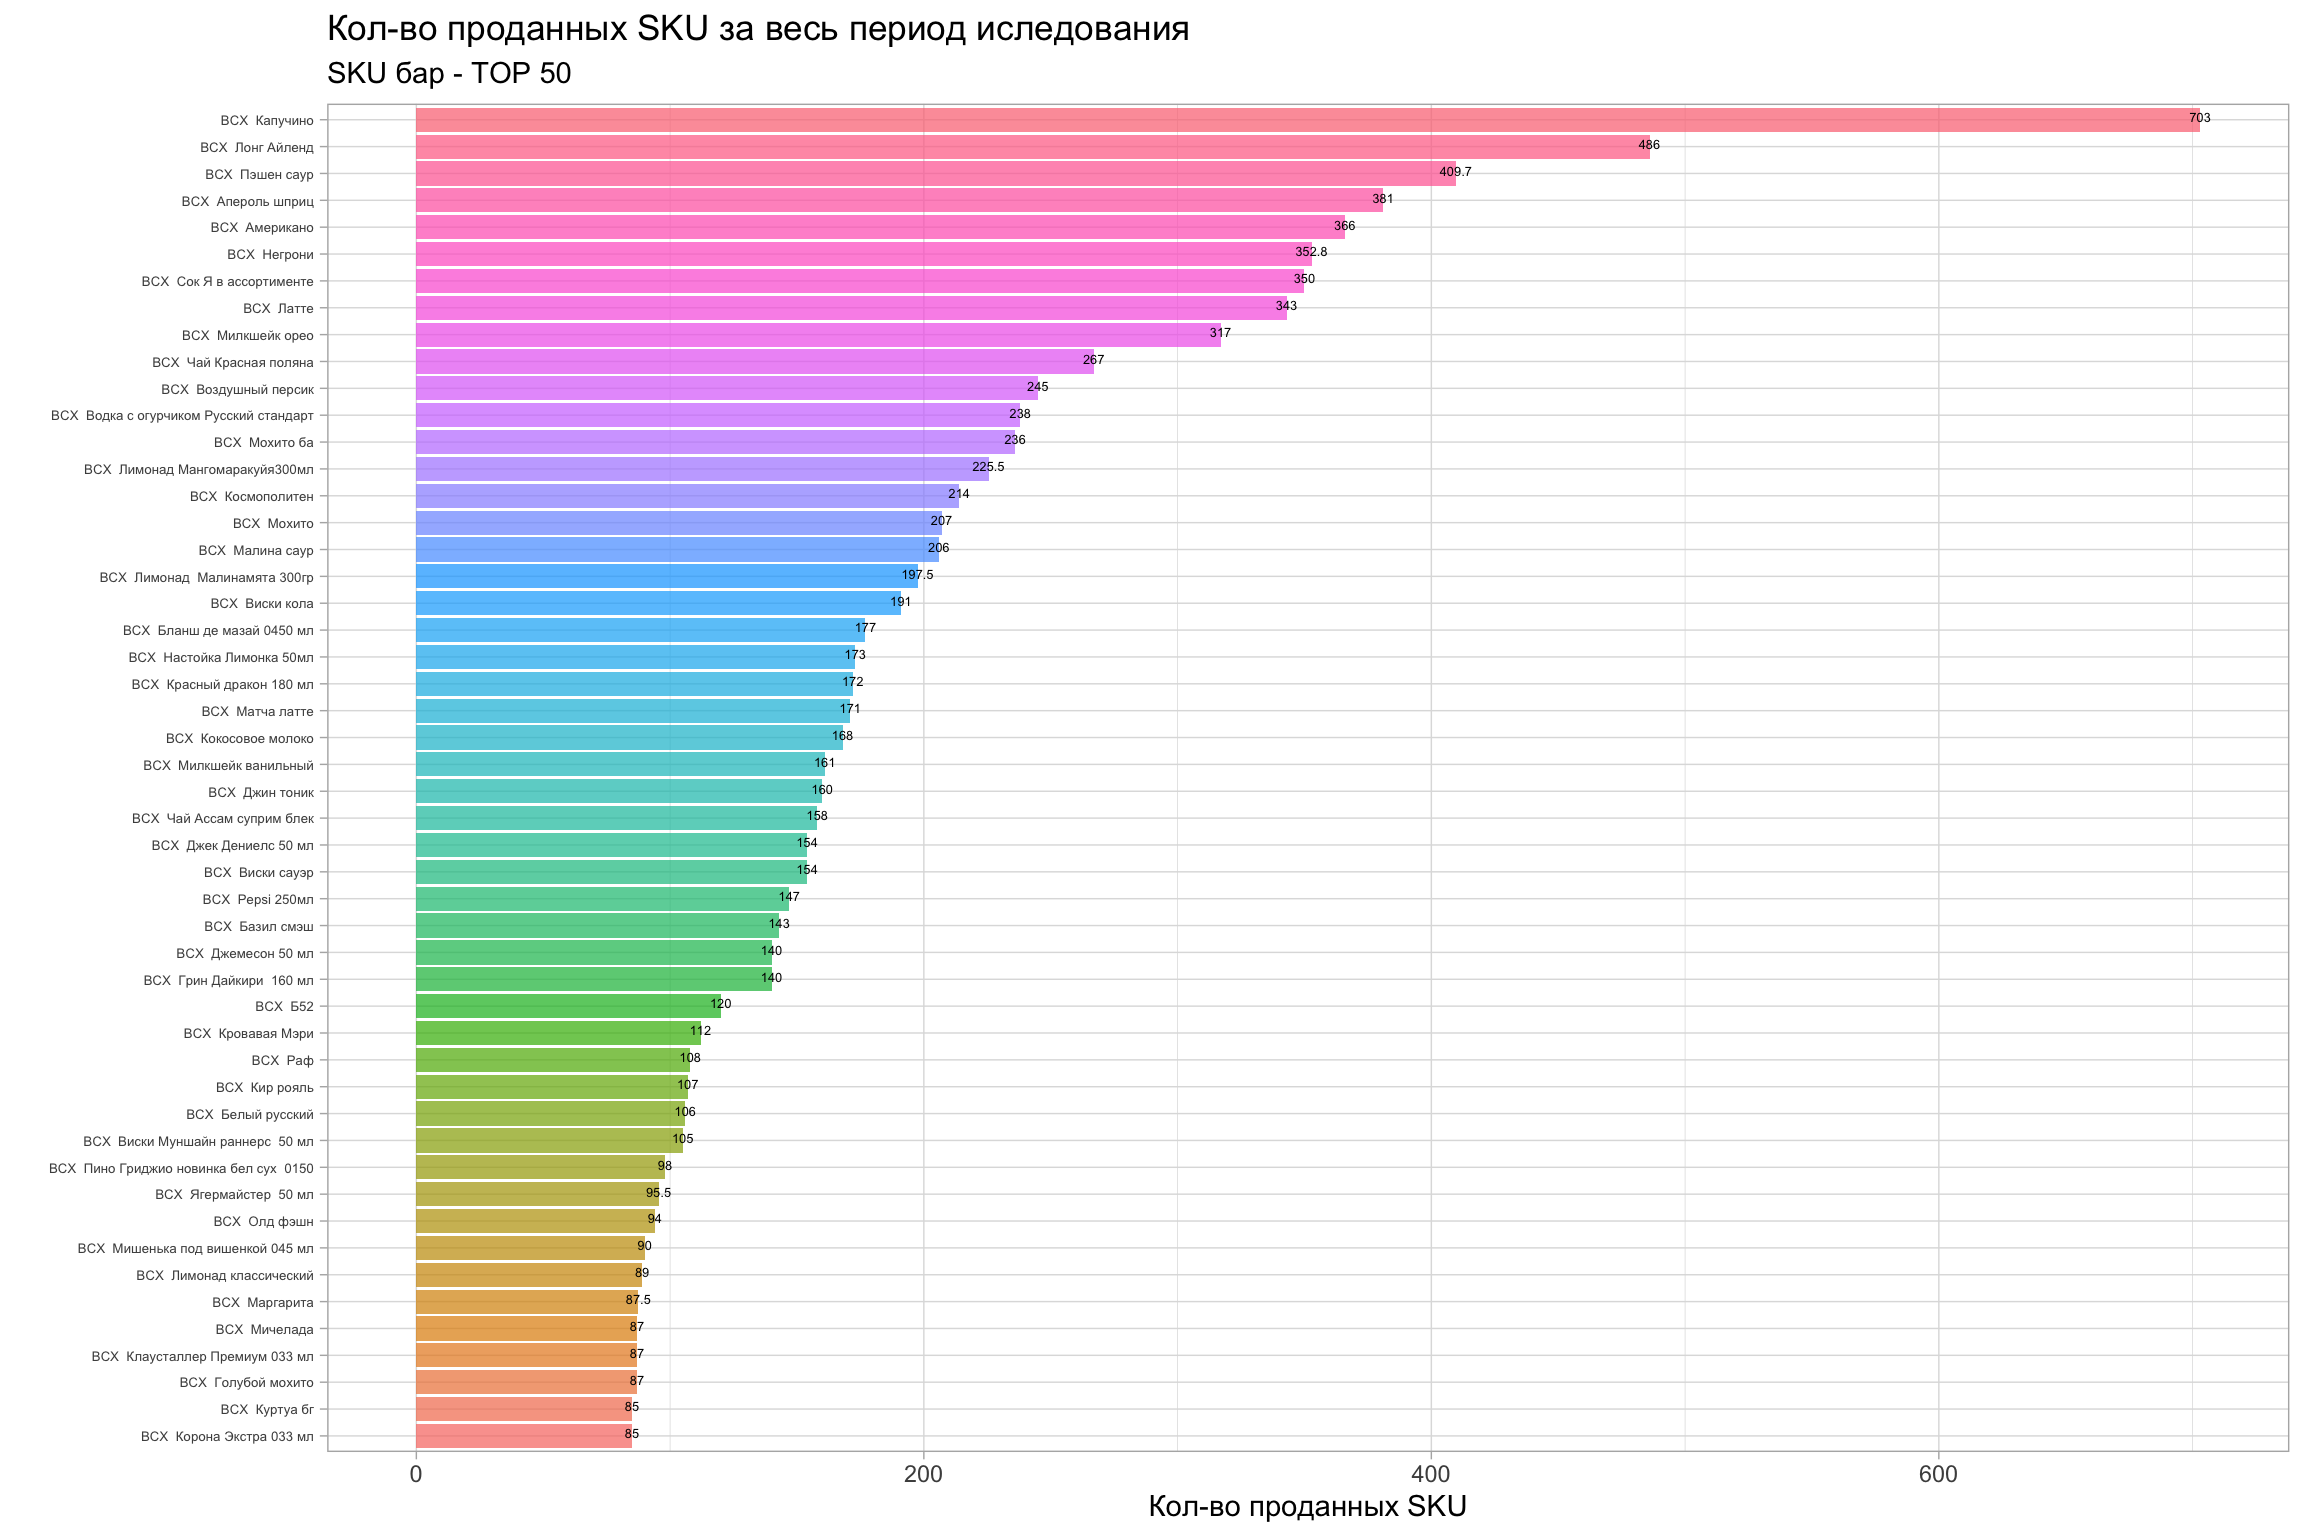
\includegraphics{./intro_files/figure-pdf/unnamed-chunk-10-1.pdf}

}

\end{figure}

\begin{tcolorbox}[enhanced jigsaw, colframe=quarto-callout-caution-color-frame, leftrule=.75mm, colback=white, arc=.35mm, toprule=.15mm, opacityback=0, bottomrule=.15mm, breakable, left=2mm, rightrule=.15mm]
\begin{minipage}[t]{5.5mm}
\textcolor{quarto-callout-caution-color}{\faFire}
\end{minipage}%
\begin{minipage}[t]{\textwidth - 5.5mm}
Данная ифонрмация представлена за весь период работы бара ``Все сейчас
хорошо''\end{minipage}%
\end{tcolorbox}

Давайте посмотрим на продажи позиций из меню за последние 3 мес. Таким
образмо, мы полчим только те SKU, которые есть в меню.

\begin{figure}

{\centering 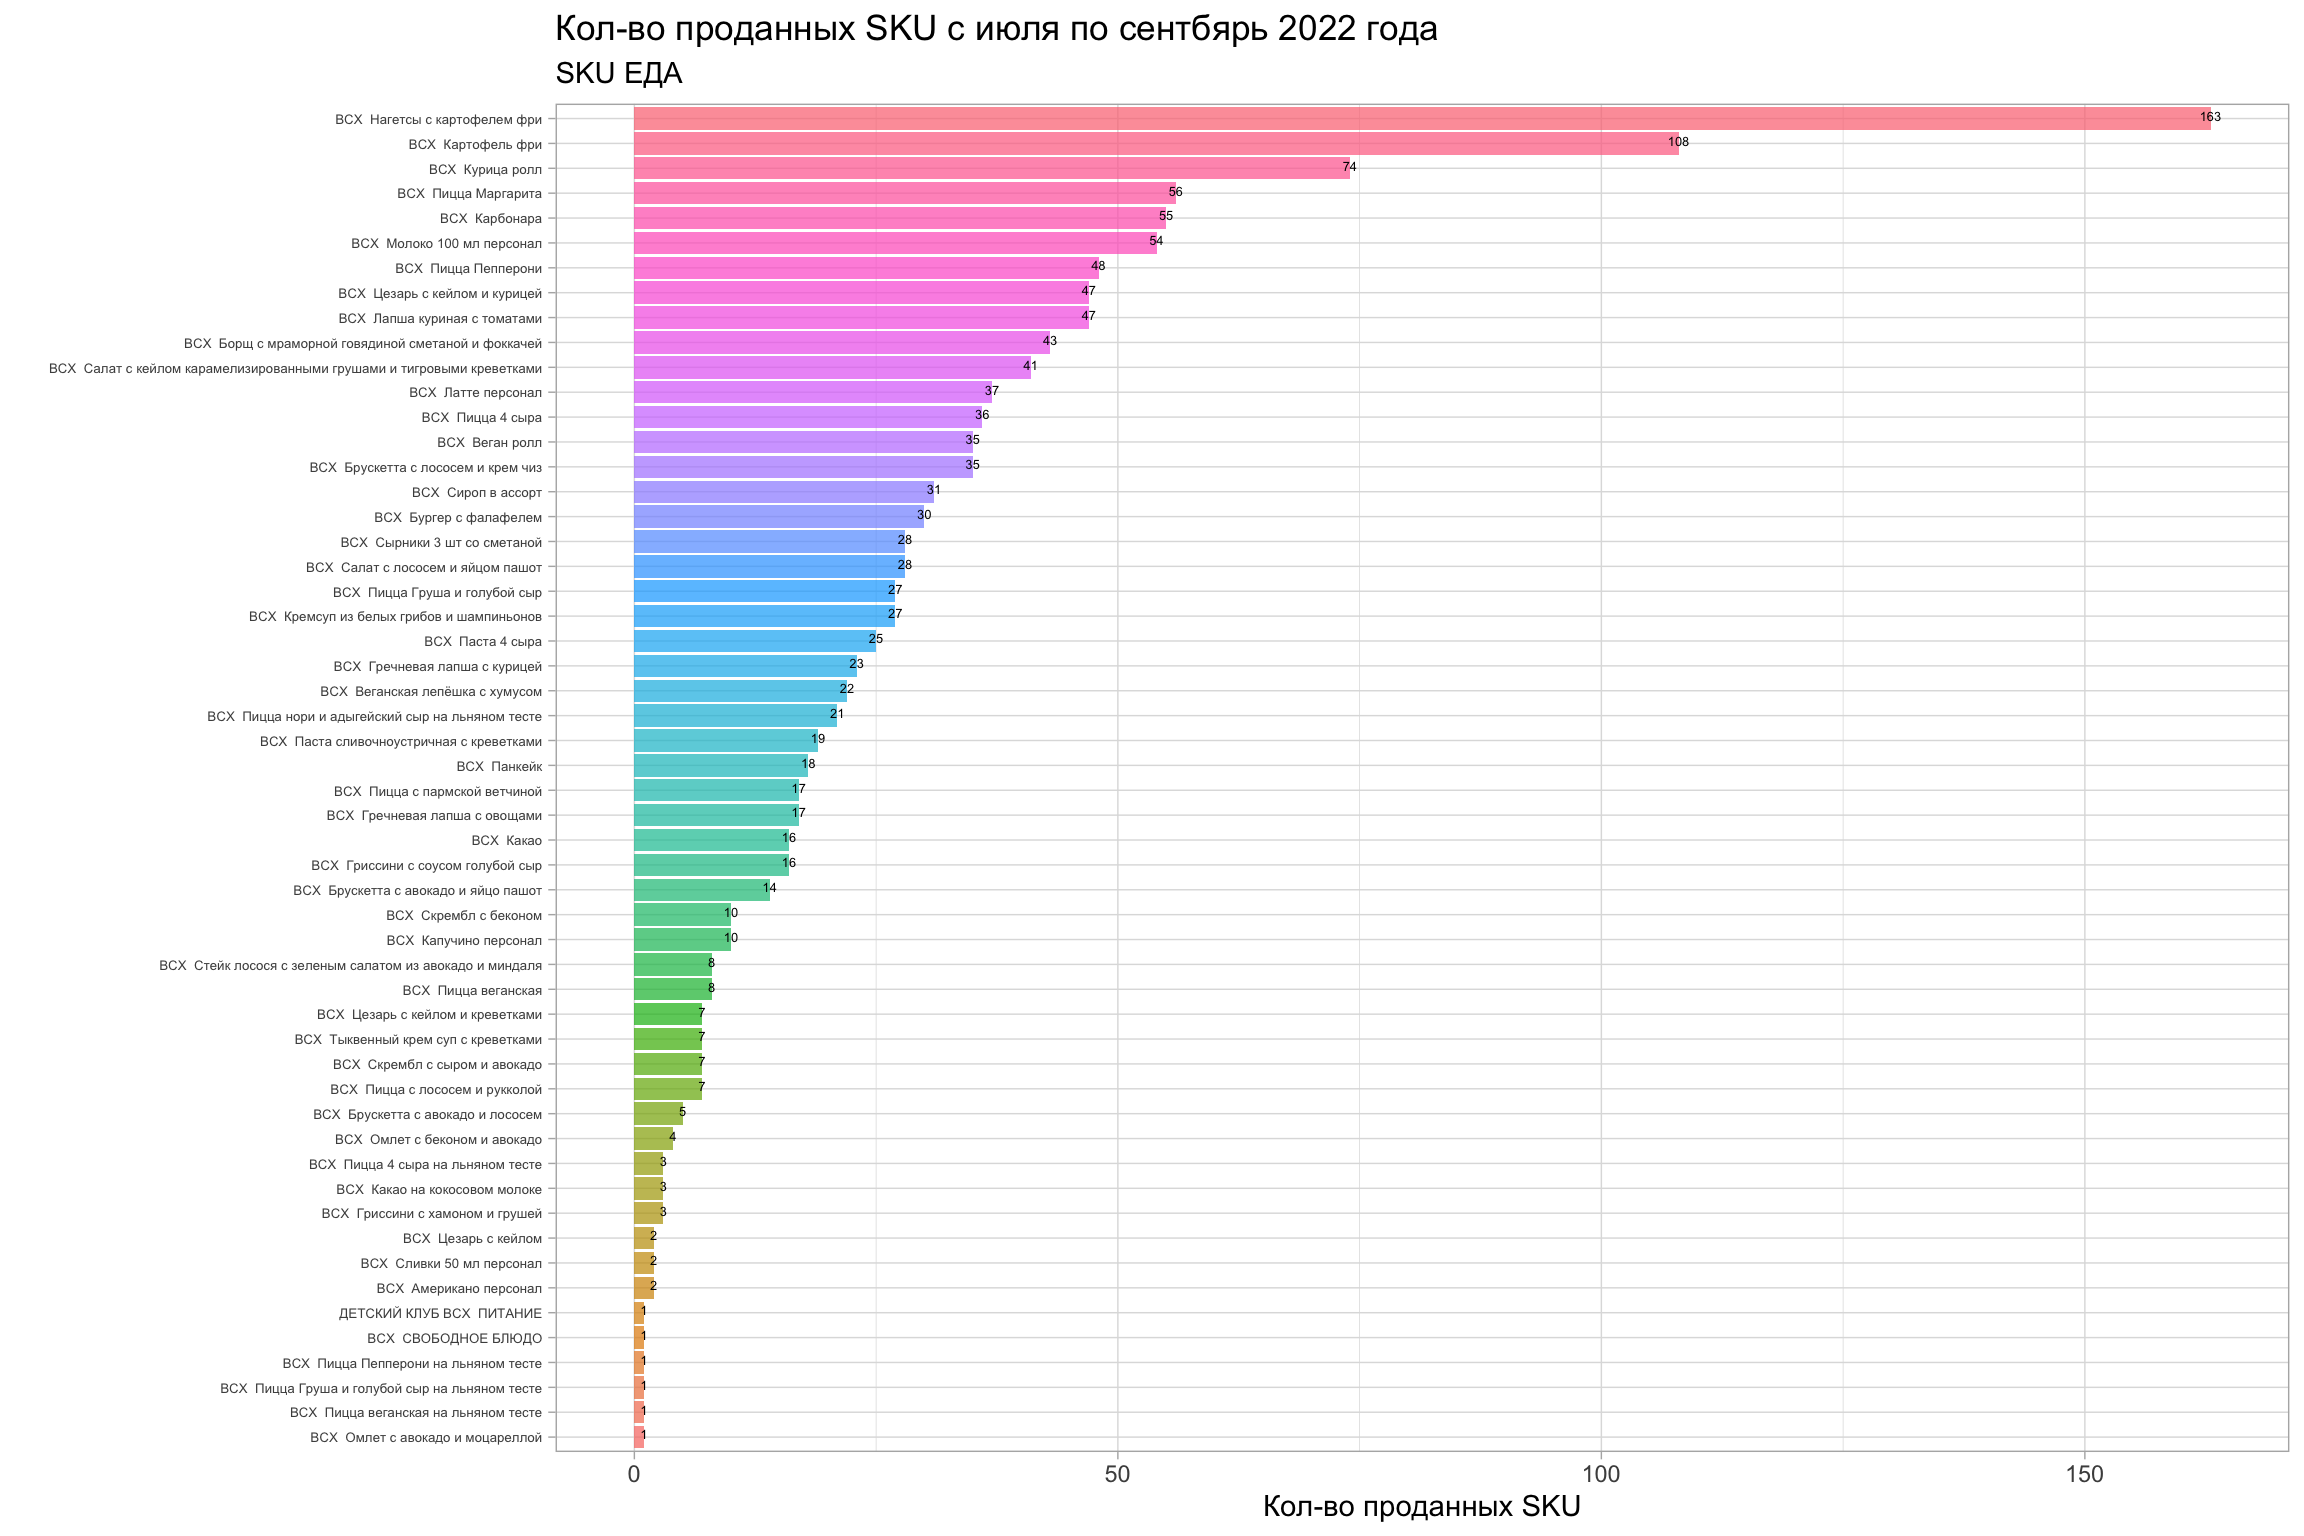
\includegraphics{./intro_files/figure-pdf/unnamed-chunk-11-1.pdf}

}

\end{figure}

Посмотрим на выручкку по этим же параметрам

\begin{figure}

{\centering 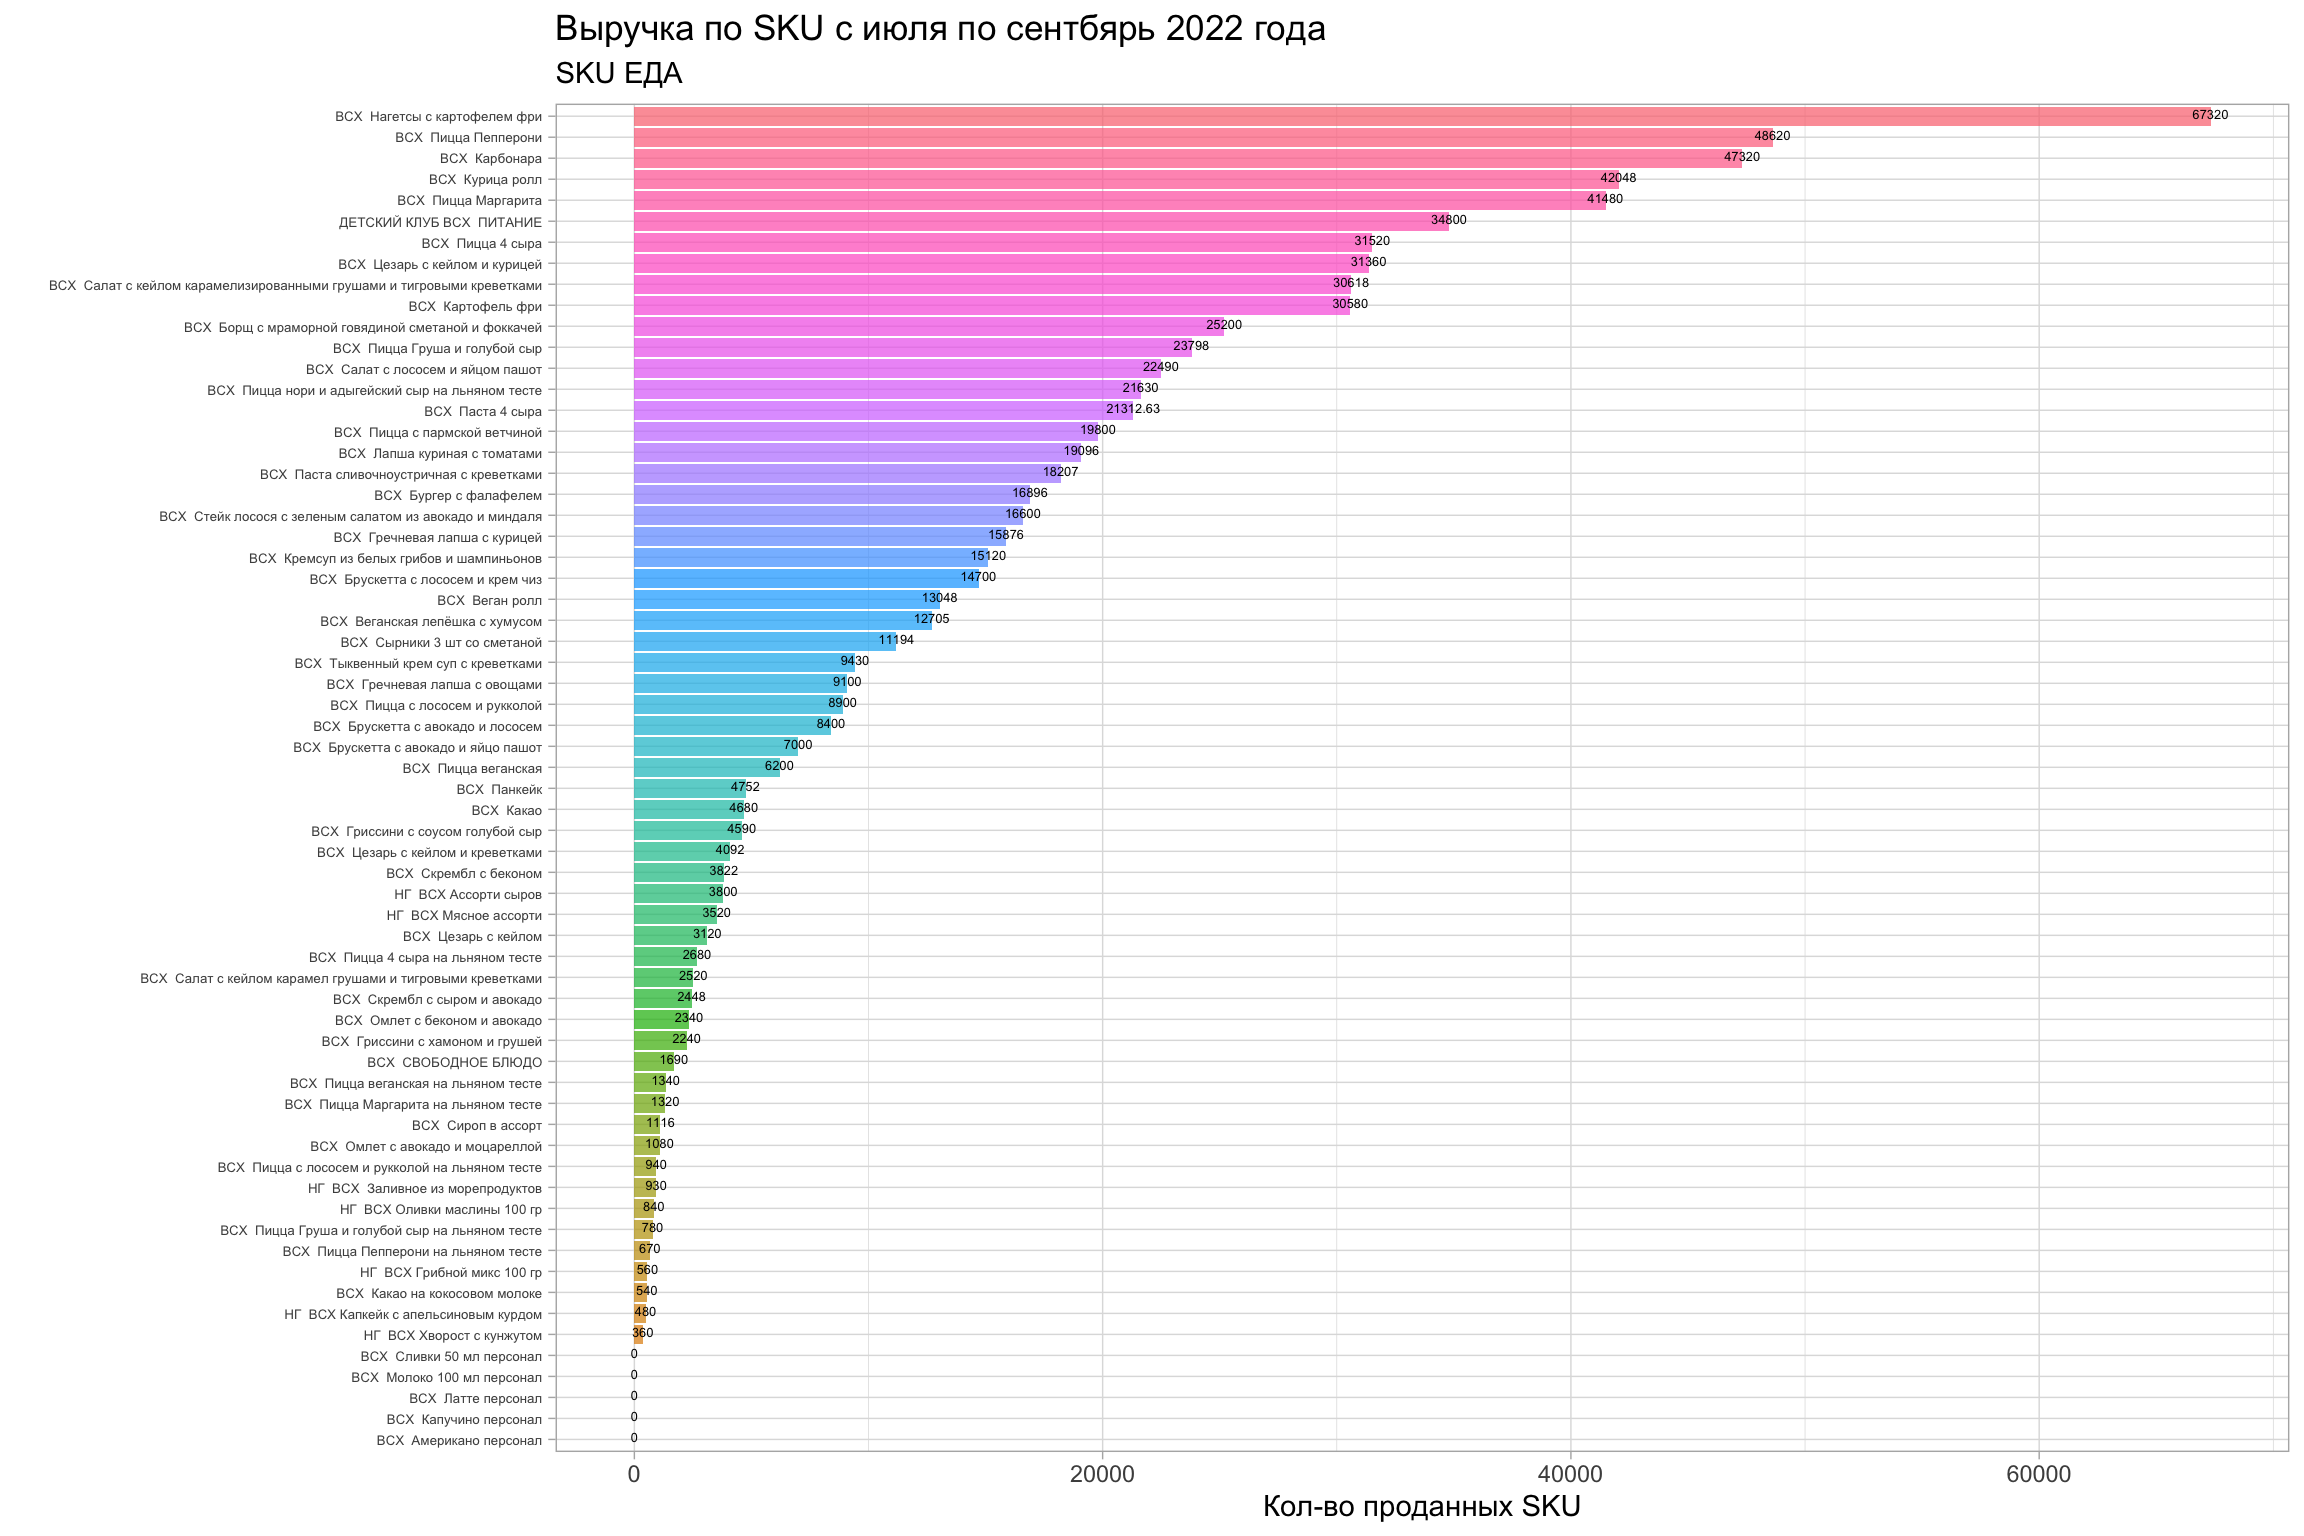
\includegraphics{./intro_files/figure-pdf/unnamed-chunk-12-1.pdf}

}

\end{figure}

Предтавим данные в таблице.

\begin{verbatim}
# A tibble: 42 x 4
   SKU                                    `Июль руб` `Август руб` `Сентябрь руб`
   <chr>                                       <dbl>        <dbl>          <dbl>
 1 ВСХ  Борщ с мраморной говядиной смета~       2800         3850           1750
 2 ВСХ  Брускетта с авокадо и яйцо пашот        1750         1400            350
 3 ВСХ  Брускетта с лососем и крем чиз          2100         9240           3360
 4 ВСХ  Бургер с фалафелем                      3696         2200           2640
 5 ВСХ  Веган ролл                              3248         2520           1680
 6 ВСХ  Веганская лепёшка с хумусом              980         2275           1400
 7 ВСХ  Гречневая лапша с курицей               3696         2520           1260
 8 ВСХ  Гречневая лапша с овощами               1400         2450            350
 9 ВСХ  Гриссини с соусом голубой сыр           1080          540           1350
10 ВСХ  Гриссини с хамоном и грушей             1120           NA            560
# ... with 32 more rows
\end{verbatim}

Судя по данным, на мой взгляд, позиции, которые выходят в ТОП, связаны с
детскими лагерями.

Отдельно рассмотрим позиции бара ``ВСХ'' за теже три месяца.

\begin{figure}

{\centering 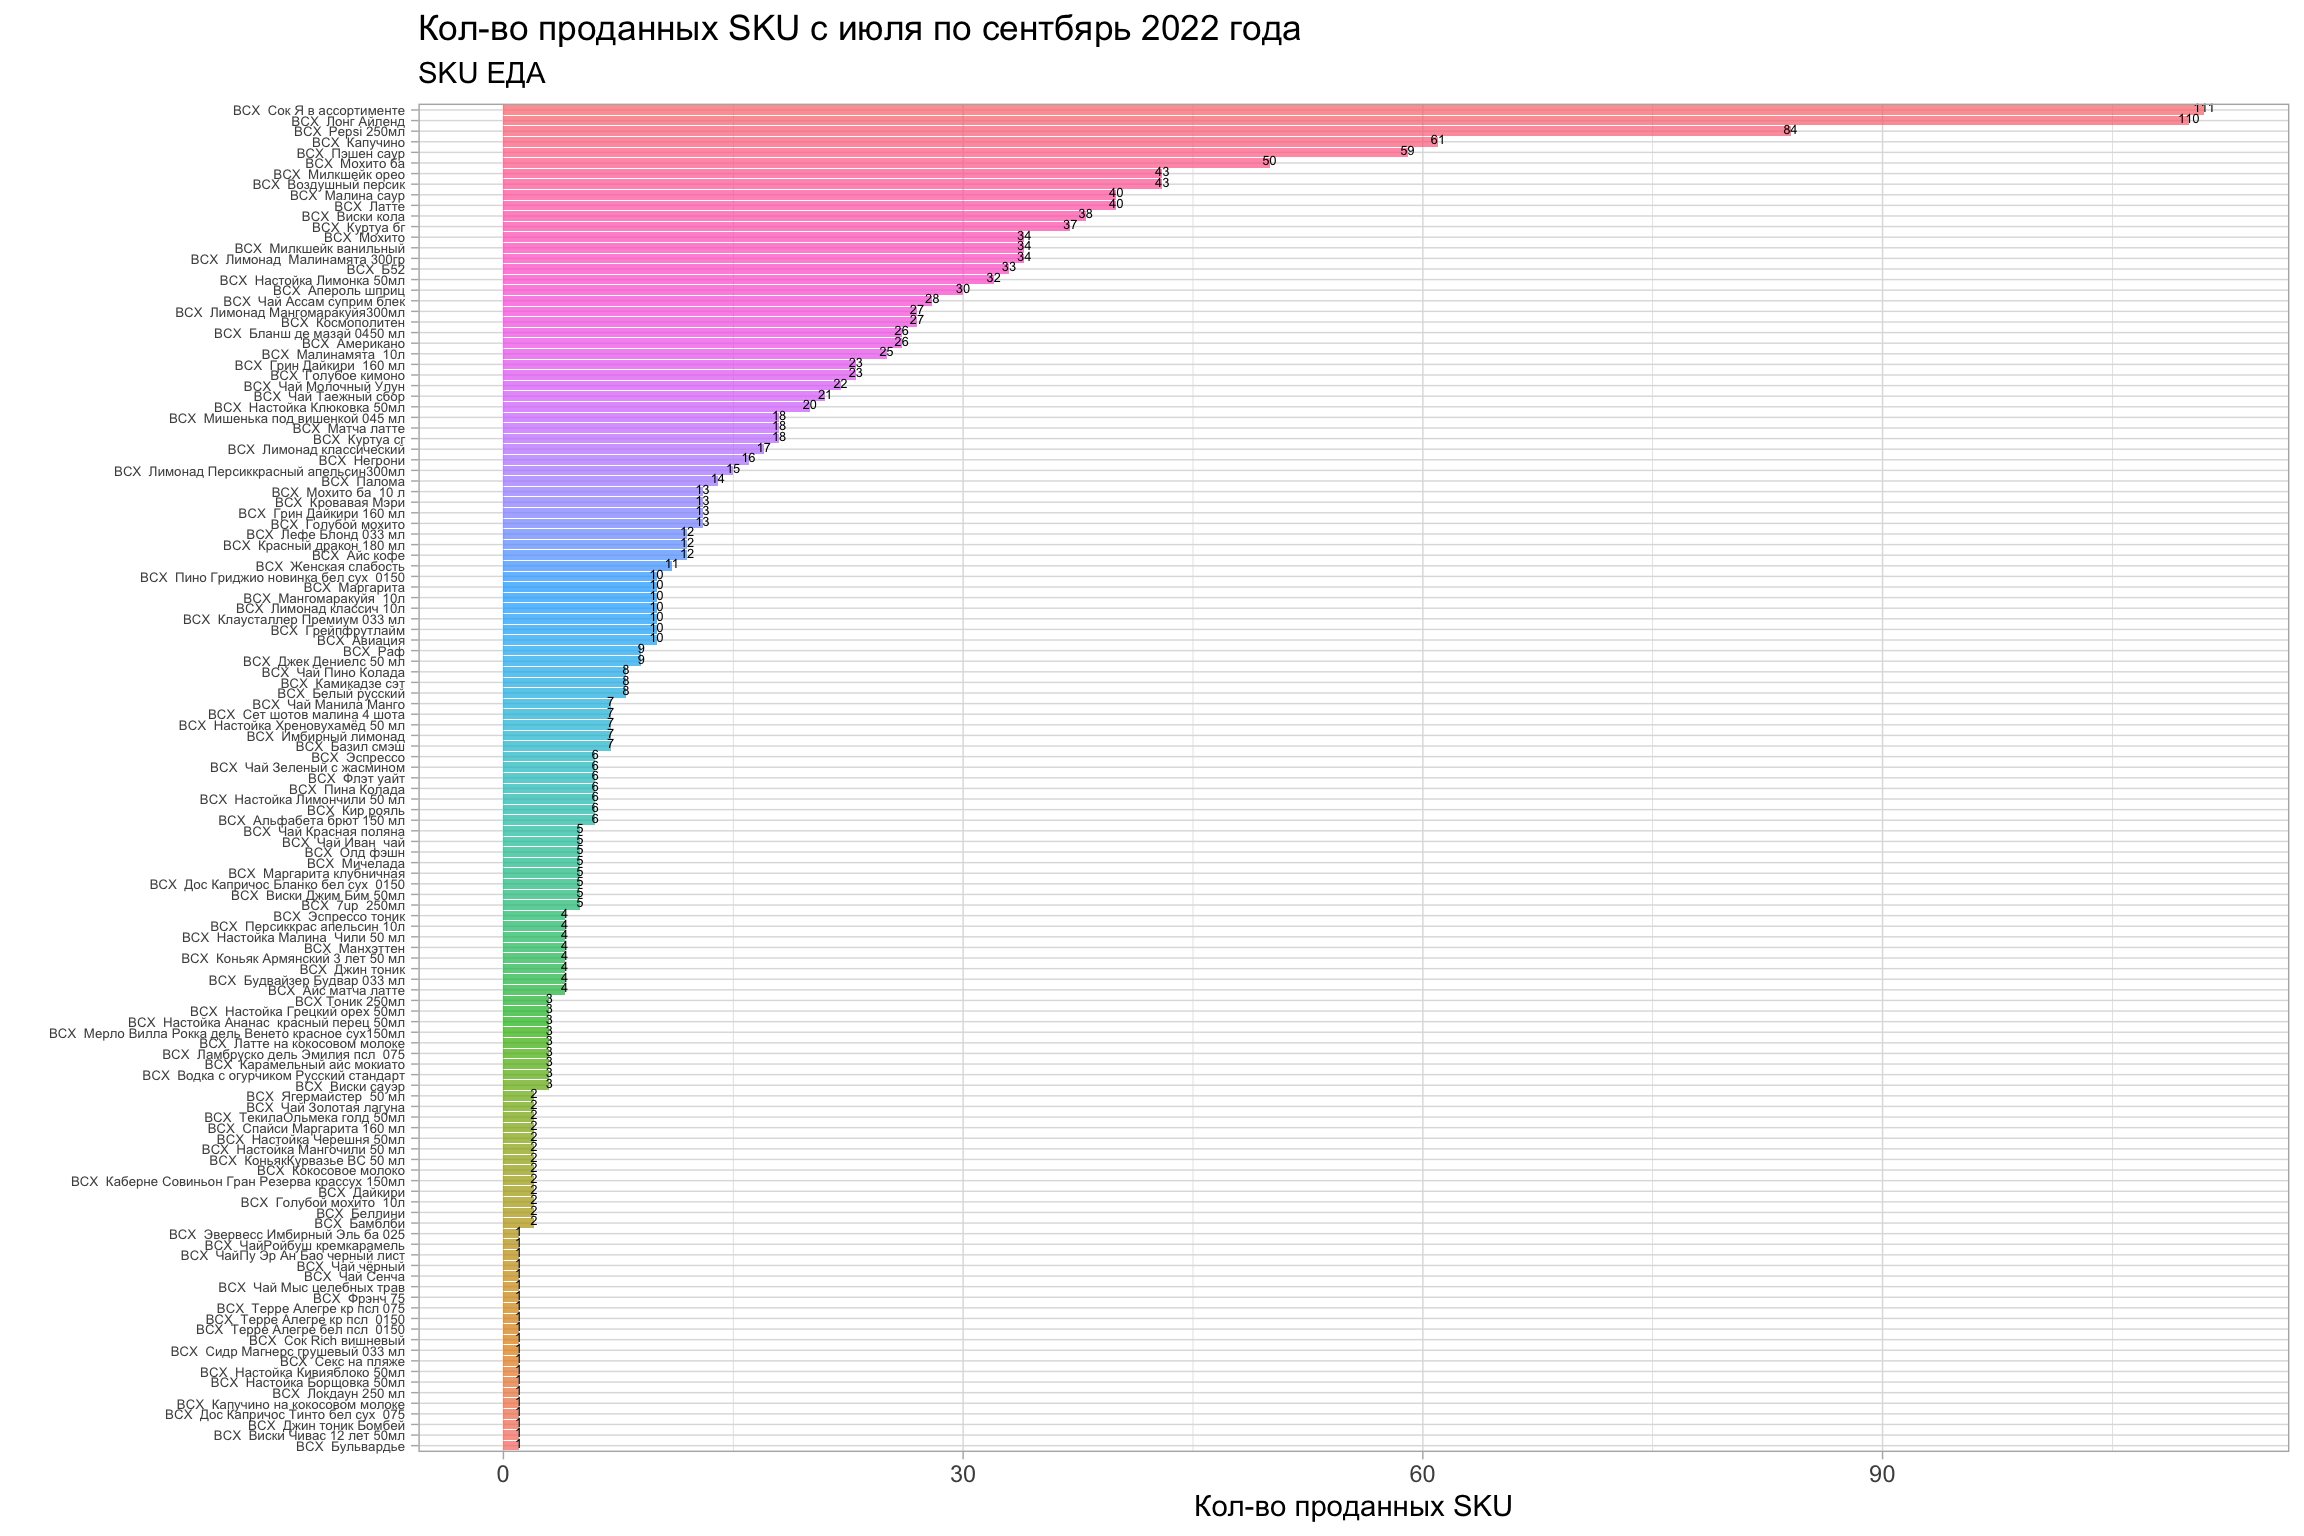
\includegraphics{./intro_files/figure-pdf/unnamed-chunk-14-1.pdf}

}

\end{figure}

Посмотрим на выручкку по этим же параметрам

\begin{figure}

{\centering 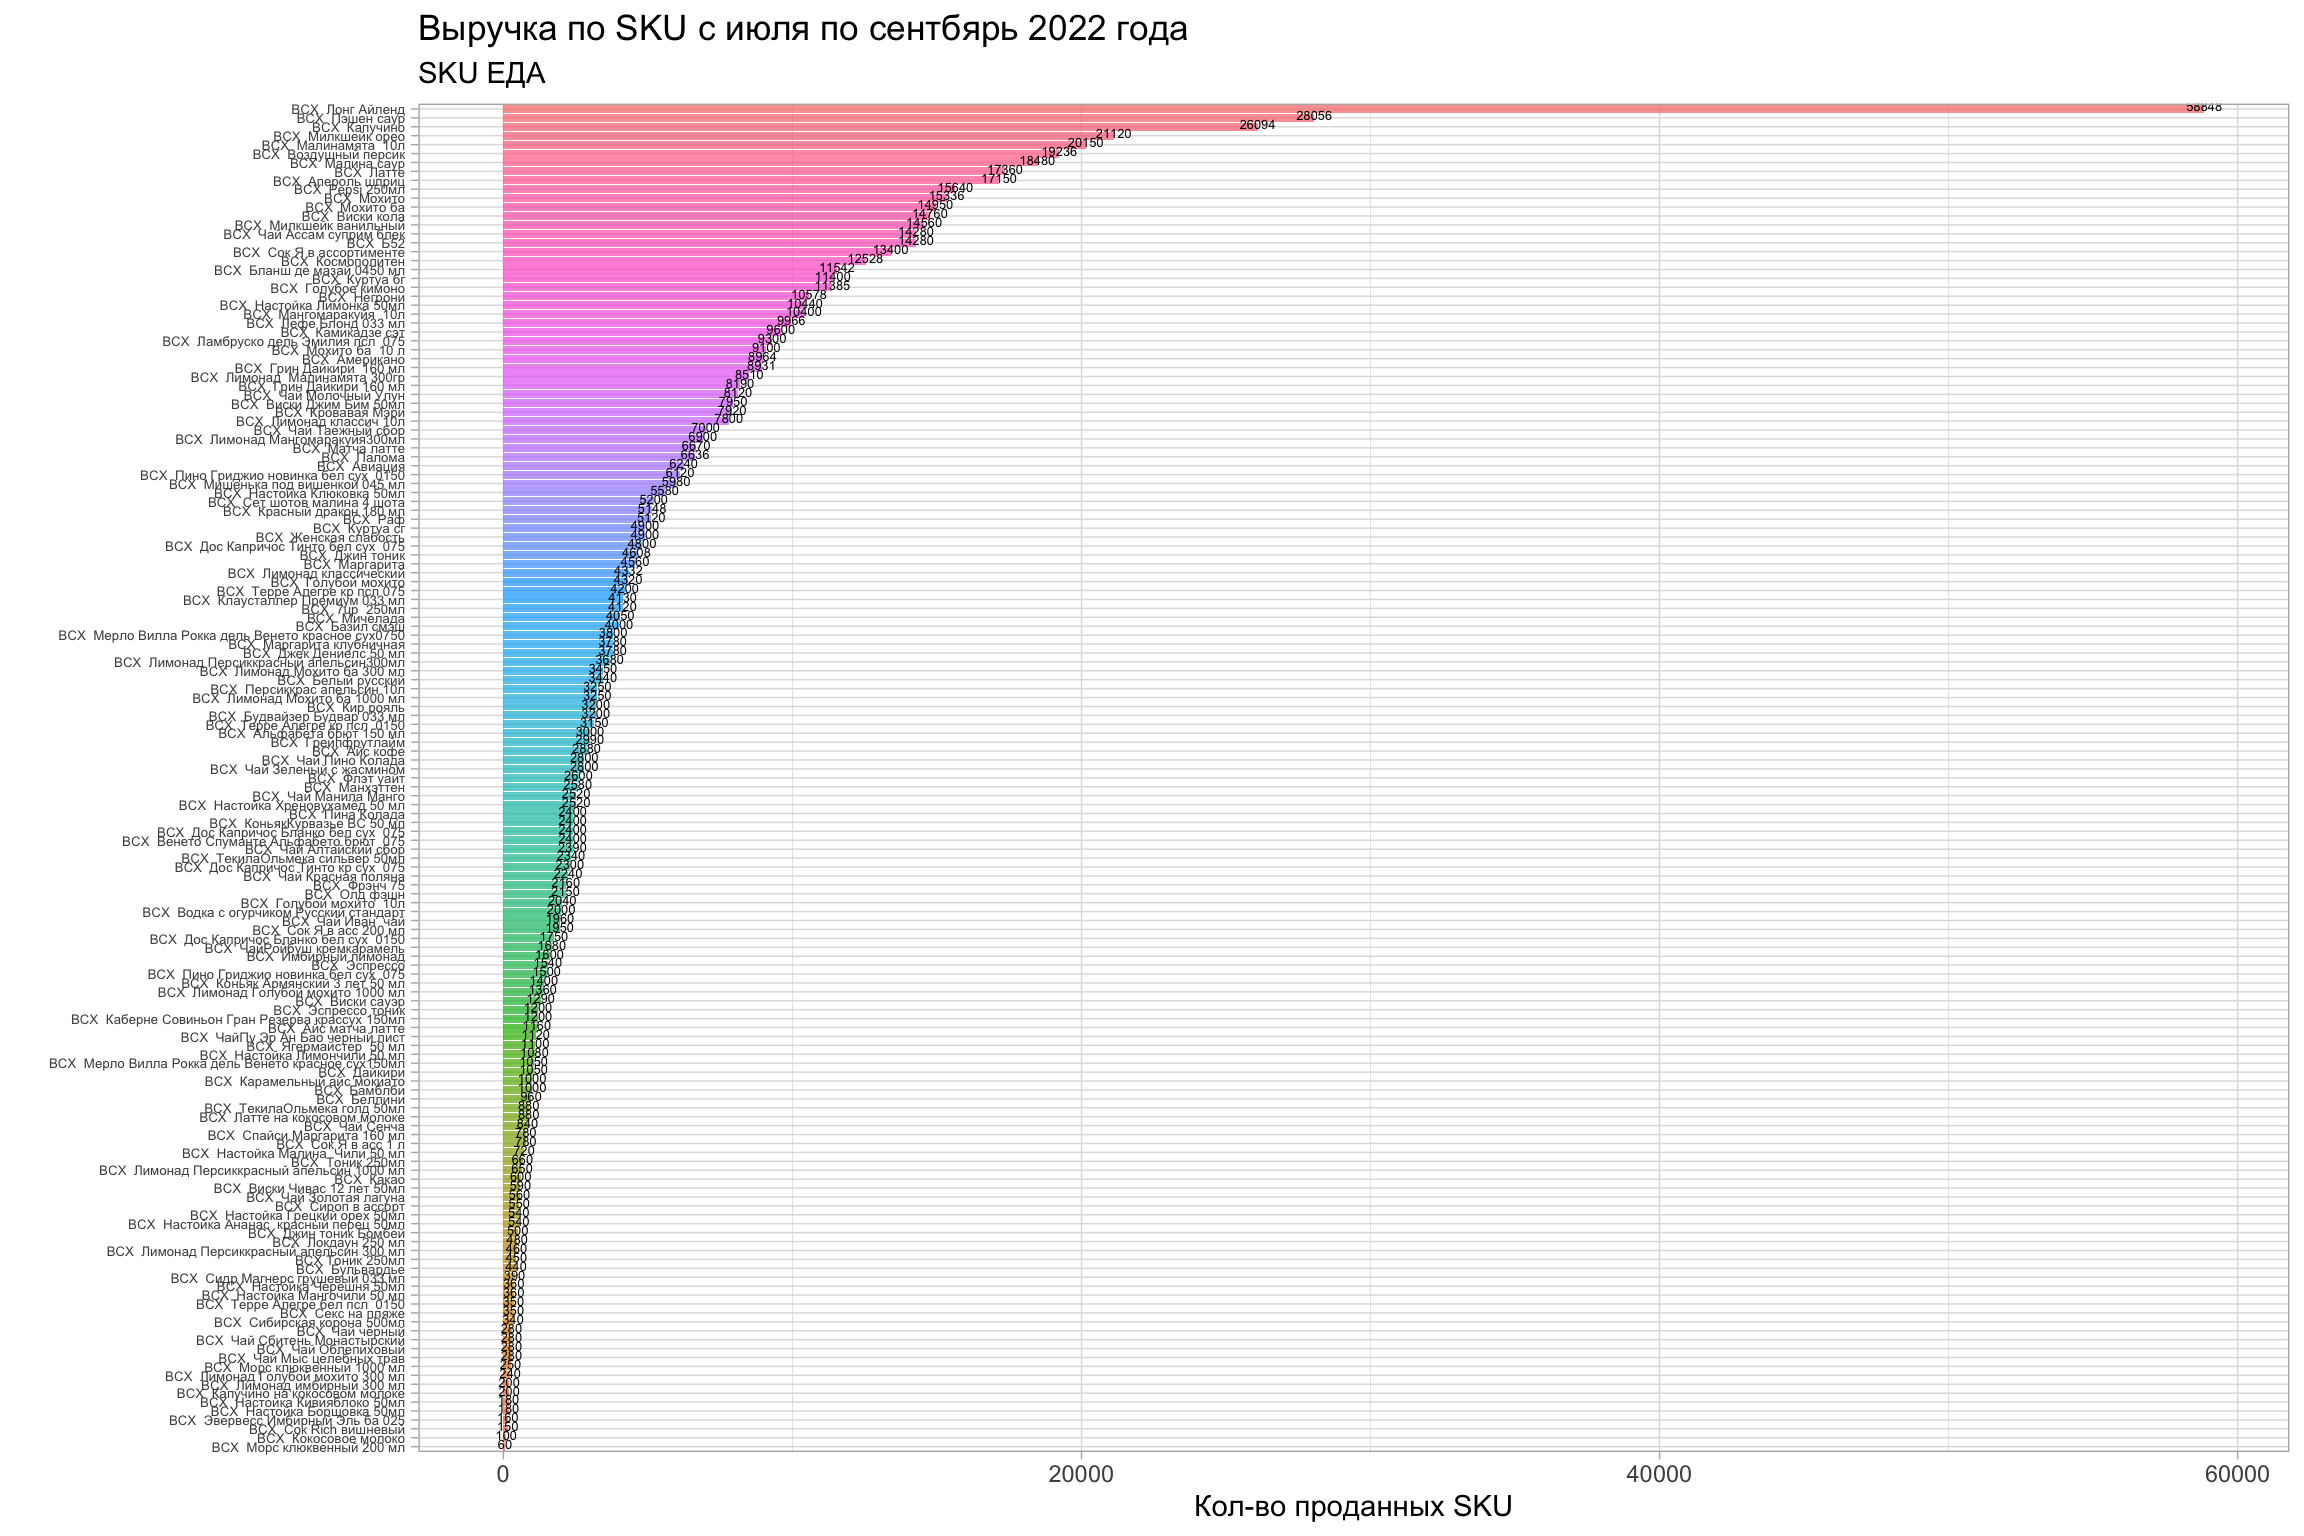
\includegraphics{./intro_files/figure-pdf/unnamed-chunk-15-1.pdf}

}

\end{figure}

Предтавим данные в таблице.

\begin{verbatim}
# A tibble: 116 x 4
   SKU                          `Июль руб` `Август руб` `Сентябрь руб`
   <chr>                             <dbl>        <dbl>          <dbl>
 1 ВСХ  Айс кофе                      1200          240            720
 2 ВСХ  Альфабета брют 150 мл          600           NA            300
 3 ВСХ  Американо                     2124          360           1260
 4 ВСХ  Апероль шприц                 5390          490           2940
 5 ВСХ  Б52                           5880           NA             NA
 6 ВСХ  Белый русский                 1200          640            800
 7 ВСХ  Бланш де мазай 0450 мл        3480          232           2320
 8 ВСХ  Будвайзер Будвар 033 мл        380          380            760
 9 ВСХ  Бульвардье                     440           NA             NA
10 ВСХ  Виски Джим Бим 50мл            780         1170             NA
# ... with 106 more rows
\end{verbatim}



\end{document}
